\begin{frame}{\underline{Problem statement}}
\section{Problem statement}
\small{To solve the ADO-DG  (\textit{Aerodynamic Design Optimization and Discussion Group}) case 6: }
\\[2mm]
\begin{itemize}
\item Objective function is to minimize $C_D$
\item $C_L$ = 0.375, Mach = 0.5
\item Baseline geometry NACA 0012 wing with semi span 3.06 units
\item  Intented to have multimodal optima
\item Geometric parameters as described in the problem
\end{itemize}

\parbox{0.38\linewidth}{
\textit\textit{{Result should highlight:}}
\begin{itemize}
\item Number of optima 
\item Geometry description of each optimal wing
\item Evidence for convergence
\item Performance value, $eb^2$, b as final span, and $e$(span efficiency factor) is defined as,
$$\boxed{
e=\frac{C_{L}^{2}}{2 \pi S C_{D}}
}$$
\end{itemize}
}
\parbox{0.57\linewidth}{
\begin{figure}
    \centering
    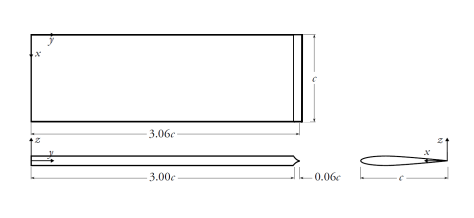
\includegraphics[scale = 0.34]{figures/baselinewing.png}
    \caption{baseline wing}
    \label{fig:baseline wing}
\end{figure}
}

\end{frame}